%% Conserved Causal Credit
%%
%% Build:
%%   pdflatex conserved-causal-credit.tex
%%   pdflatex conserved-causal-credit.tex

\documentclass[11pt]{article}
\usepackage[T1]{fontenc}
\usepackage[utf8]{inputenc}
\usepackage{lmodern}
\usepackage[margin=1in]{geometry}
\usepackage{amsmath,amssymb,amsthm}
\usepackage{booktabs}
\usepackage{array}
\usepackage{tabularx}
\usepackage{graphicx}
\usepackage{xcolor}
\usepackage{microtype}
\usepackage{xurl}
\usepackage[colorlinks=true,linkcolor=blue!55!black,
  citecolor=blue!55!black,urlcolor=blue!55!black]{hyperref}
\usepackage{tikz}
\usetikzlibrary{arrows.meta,positioning,calc,fit}
\setlength{\emergencystretch}{3em}

\newtheorem{theorem}{Theorem}[section]
\newtheorem{proposition}[theorem]{Proposition}
\newtheorem{corollary}[theorem]{Corollary}
\newtheorem{definition}[theorem]{Definition}
\newtheorem{remark}[theorem]{Remark}
\newtheorem{example}[theorem]{Example}

\newcommand{\GSLT}{\textup{GSLT}}
\newcommand{\CCC}{\textup{CCC}}
\newcommand{\Fin}{\operatorname{Fin}}
\newcommand{\Option}{\operatorname{Option}}
\newcommand{\some}{\operatorname{some}}
\newcommand{\none}{\operatorname{none}}
\newcommand{\post}{\operatorname{post}}
\newcommand{\reserve}{\operatorname{reserve}}
\newcommand{\synapse}{\operatorname{synapse}}
\newcommand{\Step}{\operatorname{Step}}
\newcommand{\Run}{\operatorname{Run}}
\newcommand{\Account}{\operatorname{Account}}
\newcommand{\Credits}{\operatorname{credits}}
\newcommand{\code}[1]{\texttt{#1}}
\newcommand{\leanname}[1]{{\scriptsize\ttfamily
  \def\_{\textunderscore\allowbreak}#1}}
\newcommand{\codepath}[1]{\nolinkurl{#1}}
\newcommand{\sem}[1]{\left[\!\left[#1\right]\!\right]}

\definecolor{processblue}{RGB}{31,84,140}
\definecolor{creditgreen}{RGB}{38,115,76}
\definecolor{signalorange}{RGB}{178,91,18}
\definecolor{boundaryred}{RGB}{150,45,45}
\tikzset{
  state/.style={draw=processblue,very thick,rounded corners=2pt,
    fill=processblue!5,align=center,inner sep=5pt,font=\small},
  resource/.style={draw=creditgreen,very thick,rounded corners=2pt,
    fill=creditgreen!6,align=center,inner sep=5pt,font=\small},
  signal/.style={draw=signalorange,very thick,rounded corners=2pt,
    fill=signalorange!6,align=center,inner sep=5pt,font=\small},
  boundary/.style={draw=boundaryred,thick,dashed,rounded corners=2pt,
    fill=boundaryred!4,align=center,inner sep=5pt,font=\small},
  flow/.style={-{Stealth[length=2.3mm]},thick}
}

\title{Conserved Causal Credit:\\
Linear-Resource Learning in Event-Driven Process Calculi}
\author{Oru\v{z}i \and Zarathustra Goertzel}
\date{August 2026 --- working paper}

\begin{document}
\maketitle

\begin{abstract}
Weighted graph-structured lambda theories make a process term and its dynamic
weight map components of one operational configuration.  This is sufficient
to place plasticity inside a calculus, but not sufficient to make the
plasticity task-sensitive.  We first give a machine-checked negative boundary:
a local saturating-add rule retains only per-synapse firing counts, so it
cannot reliably solve a representable choice task in which equally active
synapses receive different outcomes.  We then study a minimal repair,
\emph{conserved causal credit}.  A firing may create a bounded receipt naming
the participating synapse; a success event may create a bounded signal naming
its postsynaptic neuron; and a weight-changing redemption must consume both
while transferring one quantum from a fixed local credit bank.  Firing,
signaling, redemption, and expiration remain constructors of one transition
relation.  In Lean~4 we prove causal necessity and single use, donor locality,
exact conservation, bounded derived weights, finite-state admission, a
no-learning theorem for uncredited exposure, and a local diamond for
independent redemptions.  A two-choice instance learns probabilities
$(3/4,1/4)$ and later reverses them using the same four credit quanta.  We also
prove the complete semantics equivariant under independent renamings of
receipt, signal, and credit slots, so implementation slot names do not affect
the learned weights.  Finally, we compile all five action constructors into
closed terms of the undecorated reflective rho calculus: unary actions take
one ordinary communication and redemption takes three.  A syntax-level
decoder applied to the complete target term recovers its typed resource
inventory, conservation law, and derived weights exactly.  Successful finite runs
also compile to one closed control deployment, and the fail-closed compiler
emits such a deployment exactly when the source run succeeds.  A separate
closed receipt judge consumes and reissues an accepted live receipt while
emitting its addressed success signal in two ordinary communications; in the
choice canary it accepts the target receipt and rejects the reachable
distractor receipt.  We additionally prove that compiling the complete action
language through the repository's concrete cost-accounted rho syntax and then
erasing cost wrappers commutes, up to rho structural congruence, with the
direct pure-rho compiler.  Finally, an additive stochastic valuation of
indexed rho communication occurrences realizes the quantized efficacy exactly
as transition hazard.  The valuation satisfies finite sum and independent
product laws, agrees with the existing WM-PLN evidence total, and normalizes to
a race distribution under explicit finite nonzero hypotheses.  A bare target
receiver can still steal a metabolic message, but is excluded from the typed
resource-image frame.  Thus the translation gives exact operational
correspondence for compiler-generated deployments, a closed success contract,
and a constructed rate realization for receipt-observable tasks, not a
full-abstraction claim for arbitrary target contexts or arbitrary stochastic
rho environments.
\end{abstract}

\paragraph{Formal status.}
Every theorem attributed to Lean below is checked without \code{sorry}, custom
axioms, theorem stubs, or native decision shortcuts.  The development is in
\codepath{Mettapedia/MachineLearning/NeuralNetworks/LocalLearning/}; the
principal files are listed in Appendix~\ref{app:formal-map}.

\section{Introduction}
\label{sec:introduction}

Meredith's weighted graph-structured lambda theories attach a dynamic map of
weights to a rewriting configuration~\cite{meredith2026weighted}.  A rewrite
may change both the term and that map.  Consequently inference and plasticity
are two projections of one operational relation, rather than a runtime and a
separate optimizer.  This is a clean and important construction.  It answers
the architectural question ``can a process calculus contain plasticity?''
affirmatively.

It does not by itself answer the behavioral question ``does the resulting
plasticity learn a task?''  The worked rule in that construction increments a
synapse whenever its communication fires.  For fixed increment and ceiling,
the terminal weight is a function only of the synapse's initial weight and
firing count.  If two event histories have the same per-synapse counts but
different consequences, the rule cannot distinguish them.  This is not a
criticism of the weighted-\GSLT{} construction: the source paper explicitly
describes its example as a plasticity mechanism rather than a competitive
learning algorithm.  It is instead the next design question made mathematically
sharp.

The obvious repairs are not equally faithful to the process-calculus idea.
An arbitrary loss evaluator and backward error network can be encoded as more
processes, but may amount to an outer training loop wearing process syntax.
Unbounded potentiation supplies selectivity only by exhausting a ceiling.
Normalizing a global weight vector introduces a distinguished global phase.
We seek a smaller repair with four requirements:

\begin{enumerate}
\item a weight change has explicit causal evidence;
\item preference is competitive and bounded without creating credit;
\item learning remains an event of the same transition system; and
\item finite independent events retain process-style concurrency laws.
\end{enumerate}

Our proposal is to make credit a resource rather than a number added from
nowhere.  A firing produces an eligibility receipt.  A success event produces
a locally addressed signal.  Redemption requires and consumes both, and moves
one quantum from an account in the same postsynaptic neighborhood to the
eligible synapse.  The number of quanta is fixed by the state type.

\begin{center}
\resizebox{0.98\linewidth}{!}{%
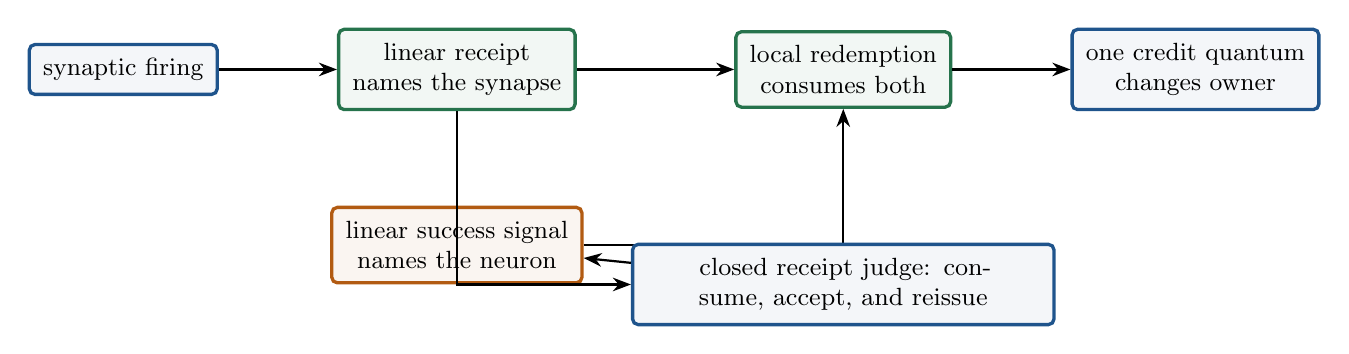
\begin{tikzpicture}[node distance=12mm and 15mm]
\node[state] (fire) {synaptic firing};
\node[resource, right=of fire] (receipt) {linear receipt\\names the synapse};
\node[signal, below=of receipt] (success) {linear success signal\\names the neuron};
\node[resource, right=20mm of receipt] (redeem) {local redemption\\consumes both};
\node[state, right=of redeem] (allocation) {one credit quantum\\changes owner};
\draw[flow] (fire) -- (receipt);
\draw[flow] (receipt) -- (redeem);
\draw[flow] (success) -| (redeem);
\draw[flow] (redeem) -- (allocation);
\node[state, below=17mm of redeem, text width=50mm] (judge)
  {closed receipt judge: consume, accept, and reissue};
\draw[flow] (receipt) |- (judge);
\draw[flow] (judge) -- (success);
\end{tikzpicture}
}
\end{center}

The word \emph{linear} in the title refers to single-use operational
resources: a receipt or signal consumed by redemption cannot be used again.
We do not claim here to embed the system in a full linear logic.  The
formalization instead proves the relevant affine and linear-use laws directly
about the transition relation.

\paragraph{Contributions.}
The paper provides the following checked boundaries and constructions.

\begin{enumerate}
\item A representability/learnability separation for count-only local
  potentiation, with both a negative reward-conditioned task and a positive
  support-aligned task.
\item A finite operational semantics for receipts, addressed success signals,
  and conserved credit allocation.
\item Exact causality, single-use, locality, conservation, boundedness, and
  no-uncredited-learning theorems.
\item A four-credit witness that learns one binary preference and then learns
  the reversed preference without increasing its budget.
\item A local diamond theorem for independent redemptions.
\item Step and run equivariance under all finite slot permutations, together
  with invariance of the observable efficacy map and a negative incoherent-
  renaming canary.
\item A concrete compiler for the complete causal action language into closed
  terms of pure rho, with exact one- or three-COMM forward simulation,
  recoverable credit observables, per-edge cost certificates, and a fused
  fail-closed deployment for every successful finite source run.
\item A closed receipt-judging success contract with exact two-COMM execution,
  a positive accepted-receipt canary, and a negative reachable rejected-
  receipt canary.
\item A positive image-context discipline and a negative ordinary-rho predator
  which locates, rather than conceals, the boundary of contextual fidelity.
\item A commuting square from the complete causal action language through the
  concrete Cost syntax to the direct pure-rho image, with both Cost endpoints
  in the runtime-supported fragment.
\item An indexed stochastic-rho valuation in which disjoint alternatives add,
  independent event families multiply, operational communication
  multiplicity is retained, and finite nonzero hazards normalize.
\item An exact rate realization of conserved-credit efficacy, with a positive
  learned-choice canary and a zero-quantum negative control.
\item An explicit boundary between the compiler-generated image proved here,
  richer autonomous domain judges, and the stronger converse modulo arbitrary
  structural-congruence detours.
\end{enumerate}

\section{Three questions that must be separated}
\label{sec:adequacy}

Learning claims often collapse representation, update information, and
reliability into one benchmark number.  We separate them before defining the
repair.

Let $K$ be a finite set of synaptic keys and let a weight map be
$w:K\to\mathbb{R}$.  A behavioral task consists of an admissibility predicate
$A(w)$, an evaluator $E(w)$, and an acceptance predicate $G(E(w))$.

\begin{definition}[Representability]
A task is \emph{representable} when
\[
  \exists w,\quad A(w)\land G(E(w)).
\]
\end{definition}

Representability prevents a failed training rule from being excused by an
insufficient hypothesis space.  It says that a legal solution exists, not
that a given update can find it.

Let a protocol $\Pi$ be a predicate on finite event histories and let
$L(h)$ be the weight map produced by a learner on history $h$.

\begin{definition}[Support-wise reliability]
The learner reliably learns a task on $\Pi$ when
\[
  \forall h,\quad \Pi(h)\Longrightarrow G(E(L(h))).
\]
\end{definition}

For a stochastic protocol this is stronger than almost-sure success: it
requires every history admitted by the declared support to solve the task.
The later finite-state admission theorem supplies a weaker recurrent notion
when support-wise reliability is too strong.

\subsection{What count-only potentiation remembers}

For synapse $k$, initial weight $w^0_k$, nonnegative increment $\eta$, ceiling
$M$, and firing count $n_k(h)$, the saturating-add rule has closed form
\[
  L_{\mathrm{count}}(h)_k
    = \min\{M,\,w^0_k+\eta n_k(h)\}.
\]

\begin{theorem}[Count sufficiency; Lean]
If two histories have the same firing count for every key, count-only
potentiation produces the same weight map.  In particular, changing reward
annotations while keeping the event-key sequence fixed is observationally
invisible to the rule.
\end{theorem}

This is \leanname{shippedAfter\_eq\_of\_fireCount\_eq} and
\leanname{shippedAfter\_ignores\_reward\_annotations}.  It is an information
theorem, not a convergence approximation.

\subsection{A task the architecture represents but the rule cannot learn}

Take two synapses, target $t$ and distractor $d$, with nonnegative admissible
weights bounded by four.  Define the target-choice probability
\[
  p_t(w)=\frac{w_t}{w_t+w_d}
\]
and accept when $p_t(w)\geq 3/4$.  The legal map $(w_t,w_d)=(3,1)$ is a witness,
so the task is representable.

The training protocol exposes each synapse twice, but only the target events
carry the success annotation.  Starting from $(1,1)$ with unit increments,
the count-only rule returns $(3,3)$ and hence $p_t=1/2$.  This is proved for
every ordering admitted by the protocol, and an explicit admitted history
refutes reliability.

\begin{theorem}[Count-only negative; Lean]
The saturating-add rule does not reliably learn the rewarded equal-exposure
choice task, although the task is representable.
\end{theorem}

The theorem is \leanname{shippedRule\_not\_reliably\_learns\_rewardedChoice}.
Its positive boundary matters equally: if the protocol fires the target twice
and the distractor zero times, the same rule reaches $(3,1)$ for every admitted
history (\leanname{shippedRule\_reliably\_learns\_supportTask}).  Thus the
result is not ``local potentiation never learns.''  It learns firing support;
it cannot learn distinctions not present in firing counts.

\section{Conserved causal credit}
\label{sec:semantics}

We now define the repair independently of any one process syntax.  This is the
operational kernel a concrete weighted-\GSLT{} presentation must refine.

Let $S$ be a finite type of synapses, $N$ a finite type of neurons, and
$\post:S\to N$ the postsynaptic endpoint map.  Fix natural numbers $R$, $G$,
and $B$ for the number of receipt slots, signal slots, and credit quanta.

\begin{definition}[Credit accounts and states]
Every credit quantum is owned either by a synapse or by a neuron's reserve:
\[
  \Account(S,N)=S+N.
\]
A core credit state is
\[
  C=(r,a),\qquad
  r:\Fin(R)\to\Option(S),\qquad
  a:\Fin(B)\to\Account(S,N).
\]
A causal-credit state adds a bounded signal bank
\[
  X=(C,g),\qquad g:\Fin(G)\to\Option(N).
\]
\end{definition}

The sum notation is implemented by constructors \code{synapse} and
\code{reserve}.  Named slots make all operations executable and make
single-use explicit.  Section~\ref{sec:symmetry} proves that their names do not
affect observable behavior under coherent renaming.

\begin{definition}[Local donor]
An account $q$ is local to target synapse $s$ when
\[
\operatorname{LocalDonor}(s,q)\;\Longleftrightarrow\;
\begin{cases}
  \post(s')=\post(s), & q=\synapse(s'),\\
  n=\post(s), & q=\reserve(n).
\end{cases}
\]
\end{definition}

Thus competition is postsynaptically local.  A target may draw from its
neuron's reserve or from another synapse arriving at the same neuron, but not
from an unrelated neighborhood.

\subsection{Actions and partial transition}

The action type has five constructors:
\[
\begin{array}{ll}
\operatorname{fire}(i,s) & \text{record firing of synapse $s$ in receipt slot $i$},\\
\operatorname{signal}(j,n) & \text{place success for neuron $n$ in signal slot $j$},\\
\operatorname{redeem}(i,j,k,s) & \text{credit synapse $s$ using all three slots},\\
\operatorname{expireReceipt}(i) & \text{discard an unused receipt},\\
\operatorname{expireSignal}(j) & \text{discard an unused signal}.
\end{array}
\]

The transition is a partial function
\[
  \delta_{\post}:X\times\operatorname{Action}\longrightarrow\Option(X).
\]
Its gates are the definition's content:

\begin{itemize}
\item \emph{Fire} succeeds only when receipt slot $i$ is empty, then writes
  $s$ there.
\item \emph{Signal} succeeds only when signal slot $j$ is empty, then writes
  $n$ there.
\item \emph{Redeem} succeeds only when receipt $i$ contains $s$, signal $j$
  contains $\post(s)$, account $a(k)$ is local to $s$, and $a(k)$ is not
  already $\synapse(s)$.  It consumes both linear resources and sets
  $a(k):=\synapse(s)$.
\item Each expiration succeeds only on an occupied slot and empties it without
  changing the allocation.
\end{itemize}

All are cases of \leanname{causalIntegratedStep}; a chronological list is
executed by \leanname{causalRun}.  There is no separate weight-update
relation.

\subsection{Derived efficacy}

The operational state is discrete, but weighted rewriting expects numerical
efficacies.  For account $q$, define
\[
  \Credits_C(q)=\left|\{k\in\Fin(B):a(k)=q\}\right|.
\]
Given base $b\in\mathbb{R}$ and quantum size $\epsilon\geq0$, the derived
weight of synapse $s$ is
\[
  w_C(s)=b+\epsilon\,\Credits_C(\synapse(s)).
\]

The weight is therefore an observation of resource ownership, not a second
mutable store that can drift from it.

\section{Causality, conservation, and the no-exposure boundary}
\label{sec:laws}

\subsection{Two resources are necessary and single-use}

\begin{theorem}[Causal redemption; Lean]
Every successful redemption of synapse $s$ from receipt slot $i$ and signal
slot $j$ satisfies all of the following:
\begin{enumerate}
\item before the step, receipt $i$ contains $s$;
\item before the step, signal $j$ contains $\post(s)$;
\item the donor account is local to $s$;
\item after the step, receipt $i$ is empty;
\item after the step, signal $j$ is empty; and
\item exactly the named credit slot is reassigned to $\synapse(s)$.
\end{enumerate}
\end{theorem}

The component results are
\leanname{causal\_redeem\_requires\_receipt},
\leanname{causal\_redeem\_requires\_signal},
\leanname{redeem\_donor\_is\_local},
\leanname{causal\_redeem\_consumes\_receipt},
\leanname{causal\_redeem\_consumes\_signal}, and
\leanname{redeem\_reassigns\_one\_credit}.

\begin{corollary}[No replay; Lean]
Neither resource used by a successful redemption can fund a second redemption.
\end{corollary}

This is \leanname{causal\_redemption\_is\_single\_use}.  Separate negative
theorems reject redemption with no receipt, no signal, a signal for another
neuron, a nonlocal donor, or a credit quantum already owned by the target.
An occupied signal slot cannot be overwritten.  These failure cases are
important: a partial transition that silently overwrote evidence would not
implement linear use.

\subsection{The weight map cannot change alone}

\begin{theorem}[One-relation integrity; Lean]
If a core transition changes the credit allocation, it also changes the
receipt state.
\end{theorem}

The result, \leanname{allocation\_change\_implies\_receipt\_change}, forbids a
successful ``map-only learning'' step in this semantics.  Signal issuance and
expiration do not themselves modify credit.  The complete state still changes
through one transition relation, but the causal witness is visible at the
boundary where ownership changes.

\subsection{Conservation and boundedness}

\begin{theorem}[Exact budget; Lean]
For every state $C$,
\[
  \sum_{q\in\Account(S,N)}\Credits_C(q)=B.
\]
\end{theorem}

This is \leanname{totalCredits\_eq\_budget}.  It follows from a finite
fiber-counting identity: allocation is a total function on exactly $B$ slots,
and the account fibers partition its domain.  The theorem holds for every
well-typed state, not merely for reachable states.

\begin{corollary}[Weight interval; Lean]
If $\epsilon\geq0$, then every synaptic weight satisfies
\[
  b\leq w_C(s)\leq b+\epsilon B.
\]
\end{corollary}

The upper and lower bounds are
\leanname{derivedWeight\_upper\_bound} and
\leanname{derivedWeight\_lower\_bound}.  Unlike saturating addition, the
upper bound does not require a special ceiling operation: it is a consequence
of competition for a conserved supply.

\subsection{Exposure is not credit}

Call firing and receipt expiration \emph{structural} actions; neither redeems
credit.

\begin{theorem}[No uncredited learning; Lean]
Every successful finite run consisting only of structural actions preserves
the entire allocation and hence every derived synaptic weight.
\end{theorem}

These are \leanname{structural\_run\_preserves\_allocation} and
\leanname{structural\_run\_preserves\_derivedWeight}.  This is the repaired
system's negative boundary: traffic can create and remove eligibility, but
traffic alone is not declared successful learning.

\section{The smallest learning-and-reversal witness}
\label{sec:canary}

The exact canary uses two synapses $t,d$ sharing one postsynaptic neuron, one
receipt slot, one signal slot, and four credit quanta.  Initially
\[
  a_0=\synapse(t),\quad a_1=\synapse(d),\quad
  a_2=a_3=\reserve(\ast).
\]
With $b=0$ and $\epsilon=1$, the weights are the credit counts.

\begin{center}
\small
\begin{tabular}{@{}lcccc@{}}
\toprule
Phase & target credits & distractor credits & $(w_t,w_d)$ & accepted behavior\\
\midrule
initial & 1 & 1 & $(1,1)$ & neither $3/4$ task\\
equal exposure, no redemption & 1 & 1 & $(1,1)$ & target task fails\\
two target redemptions & 3 & 1 & $(3,1)$ & $p_t=3/4$\\
two later distractor redemptions & 1 & 3 & $(1,3)$ & $p_d=3/4$\\
\bottomrule
\end{tabular}
\end{center}

Each credited firing is followed by a matching success event and redemption.
Each uncredited firing is followed by receipt expiration.  In the reversal
phase, the distractor does not draw from a freshly enlarged reserve: it takes
the same two quanta that the target previously acquired.  Total credit is four
in all three named states.

\begin{theorem}[Learning and relearning; Lean]
The explicit-signal causal run satisfies all of the following:
\begin{enumerate}
\item the uncredited equal-exposure episode returns the initial state;
\item the target-credit episode returns the $(3,1)$ state;
\item that state solves the target $3/4$ task;
\item the concatenated target-then-reverse run returns the $(1,3)$ state; and
\item the final state solves the reversed distractor $3/4$ task.
\end{enumerate}
\end{theorem}

The conjunction is checked as
\leanname{causal\_credit\_learns\_and\_relearns}.  The run equalities are
evaluated by Lean's kernel.  The example is deliberately minimal.  It proves
that the mechanism can implement task-sensitive preference and reversal under
a fixed budget; it does not estimate sample efficiency or establish that a
particular closed environment will generate the scripted success events.

\section{Independent credit events commute}
\label{sec:diamond}

An event-driven learner must say what concurrent independent updates mean.
Two redemptions are slot-independent when their receipt slots, signal slots,
and credit slots are pairwise distinct.  Synapses need not be distinct: the
criterion is resource separation.

Let $E_{i,j,k,s}$ denote the total state effect of an already-enabled
redemption: consume receipt $i$, consume signal $j$, and assign credit slot
$k$ to $s$.

\begin{theorem}[Effect commutation; Lean]
If $(i_1,j_1,k_1)$ and $(i_2,j_2,k_2)$ are pairwise distinct coordinatewise,
then for every complete state $X$,
\[
 E_{i_2,j_2,k_2,s_2}(E_{i_1,j_1,k_1,s_1}(X))
 =
 E_{i_1,j_1,k_1,s_1}(E_{i_2,j_2,k_2,s_2}(X)).
\]
\end{theorem}

This is \leanname{redemptionEffect\_commutes}.  The proof is not merely about
the derived weights.  It establishes equality of the receipt functions,
signal functions, and allocation functions by commutation of updates at
distinct positions.

\begin{theorem}[Operational diamond; Lean]
If both independent redemptions are enabled in $X$, executing them in either
order succeeds and produces the same state.
\end{theorem}

The theorem \leanname{independent\_redemptions\_form\_diamond} combines effect
commutation with
\leanname{redemptionEffect\_preserves\_independent\_enabling}.  It is a local
diamond, not a claim of global confluence: overlapping redemptions compete for
resources and may intentionally disable one another.

This distinction is useful for implementations.  Independent events may be
scheduled or batched in either order without changing semantics.  Conflicting
events require the ordinary nondeterministic choice of the process system.

\section{Slot names are not learning data}
\label{sec:symmetry}

Finite arrays make the semantics executable, but named resource slots can
create artificial state distinctions.  Before quotienting states by those
names, we prove the stronger operational fact needed to justify the quotient.

Let $\rho$, $\sigma$, and $\kappa$ be permutations of receipt, signal, and
credit slots.  Reindex a bank $f$ by
\[
  (\pi_\ast f)(j)=f(\pi^{-1}(j)).
\]
Relabel a state by reindexing all three banks, and relabel an action by applying
the corresponding permutation to every slot it mentions.

\begin{theorem}[One-step equivariance; Lean]
For every state $X$ and action $u$,
\[
  \delta_{\post}((\rho,\sigma,\kappa)_\ast X,
                  (\rho,\sigma,\kappa)_\ast u)
  =
  \Option.map((\rho,\sigma,\kappa)_\ast,
              \delta_{\post}(X,u)).
\]
The equality covers both successful and rejected actions.
\end{theorem}

This is \leanname{causalIntegratedStep\_relabel}.  Its relational form is
\leanname{CausalStep\_relabel\_iff}.

\begin{theorem}[Run equivariance; Lean]
Coherent relabeling commutes with every finite chronological history, including
histories that fail partway through.
\end{theorem}

The result is \leanname{causalRun\_relabel}.  The proof is an induction using
the exact one-step equality, not a post-hoc statement about terminal weights.

\begin{corollary}[Observable invariance; Lean]
For every account $q$, credit ownership counts are invariant under credit-slot
permutation.  Consequently the complete real-valued derived weight map is
invariant under arbitrary receipt and credit permutations.
\end{corollary}

These are \leanname{accountCredits\_relabelCore} and
\leanname{derivedWeight\_relabelCore}.  Thus the representation contains
labeled copies, but the learning observable depends only on their ownership
multiset.

The coherence condition is essential.  A checked two-slot counterexample has
slot zero occupied and slot one empty.  Swapping the state's receipt slots but
not the action changes a firing aimed at slot zero from rejected to enabled
(\leanname{state\_only\_receipt\_swap\_changes\_behavior}).  Coherently
swapping both preserves rejection
(\leanname{coherent\_receipt\_swap\_preserves\_rejection}).  The correct
symmetry acts on the operational presentation, not on an isolated state.

\section{Finiteness and recurrent reliability}
\label{sec:finite}

When $S$ and $N$ are finite, every component of the causal-credit state is a
function between finite types.  The state and action spaces are therefore
finite (\leanname{causalState\_finite} and \leanname{creditAction\_finite}).
This makes exhaustive graph construction possible, but finiteness alone does
not imply learning.

The companion admission theory treats an unlabelled finite transition
relation.  A support run is fair when every edge enabled infinitely often is
taken infinitely often.  An infinitely recurring set of a fair run forms a
closed strongly connected bottom class.  Let a good predicate describe
accepted behavior.

\begin{definition}[Bottom admission]
An initial state is bottom-admissible for $G$ when every reachable bottom
class is contained in $G$.
\end{definition}

\begin{theorem}[Finite bottom-class soundness; Lean]
For a finite state type, bottom admission implies that every fair support run
recurrently satisfies the good predicate.
\end{theorem}

The generic result is
\leanname{bottomAdmissible\_implies\_fairlyReliable}.
Its causal-credit specialization is
\leanname{bottomAdmission\_sound\_for\_causalCredit}.  A positive finite canary
has one good terminal bottom class.  A negative branching canary has a
reachable bad sink and is rejected.  Hence the admission criterion does not
turn finiteness into a vacuous success proof.

This layer supplies a terminating verification problem for any concrete
finite environment/learner composition: construct its reachable graph,
identify bottom classes, and check the task on all of them.  The present paper
does not yet provide the closed environment required for that final check.

\section{State identity is part of the semantics}
\label{sec:identity}

Eligibility and success resources matter only if configuration identity
retains them.  A simulator that hashes a marking and weight map while omitting
its trace can merge states with different legal futures.

The formal state-identity canary uses timing states with a marking, weight,
optional trace, and clock.  Two states with equal marking and weight but
different trace have the same reduced key and different next weights.  Adding
trace but omitting time still fails.  The full key is injective and therefore
adequate for every observable
(\leanname{shippedTimingKey\_not\_adequate},
\leanname{traceTimingKey\_not\_adequate}, and
\leanname{fullTimingKey\_adequate}).

There is a genuine tradeoff: the full key has infinite range when the clock is
real-valued (\leanname{fullTimingKey\_range\_infinite}).  Exact finite-state
admission therefore requires bounded or discretized trace/time state, not
merely an implementation that forgets it.  The conserved-credit construction
chooses bounded discrete banks precisely so the Markov state remains explicit
and finite.

\section{Internalization in the undecorated rho calculus}
\label{sec:rho-internalization}

The resource semantics above is not a new primitive required of the host
calculus.  We now give a concrete compiler into ordinary rho communication,
following the general observation that cost-accounted rho can be represented
inside undecorated rho by messages on metabolic channels
\cite{meredith2026mortal}.  The result is deliberately stated at the strength
proved by the formal artifact: exact forward simulation on compiler-generated
terms, together with an explicit boundary on target contexts.

Let $C$ be the finite type of all observable resource states: empty and full
receipt slots, empty and full signal slots, and each credit slot paired with
its current account.  A finite enumeration gives an injective code
$\nu:C\hookrightarrow\mathbb{N}$.  For every $n$, let $M_n$ be a closed marker
process containing exactly $n$ rho input/output nodes, and define

\[
  m(c)=@M_{\nu(c)}, \qquad R(c)=m(c)!(0).
\]

The input/output count is invariant under structural congruence.  Consequently
$m(c)\equiv m(c')$ implies $c=c'$; different resource states cannot collapse
merely because their names are quoted processes.  Each $R(c)$ is a closed,
well-sorted term of the authored pure-rho carrier.

Four action forms replace one resource state by another.  Their common
compiler schema is

\[
 R(c)\;\mid\;
 \operatorname{for}({-}\leftarrow m(c))\{R(c')\}
 \quad\longrightarrow\quad R(c').
\]

Firing changes an empty receipt to a receipt naming its synapse; signaling
changes an empty signal slot to one naming its neuron; and the two expiration
actions return their occupied slots to empty.  Each takes exactly one ordinary
COMM step.

Redemption is a three-resource transaction.  If $r$, $s$, and $d$ denote the
occupied receipt, success signal, and donor-credit channels, its compiled
handler is the nested input

\[
 \operatorname{for}({-}\leftarrow m(r))\{
 \operatorname{for}({-}\leftarrow m(s))\{
 \operatorname{for}({-}\leftarrow m(d))\{
   R(r_0)\mid R(s_0)\mid R(d')
 \}\}\},
\]

where $r_0$ and $s_0$ are the corresponding empty-slot states and $d'$ assigns
the selected quantum to the credited synapse.  In parallel with the three
resource messages this handler takes exactly three COMM steps.  An arbitrary
untouched frame is preserved throughout.

\begin{theorem}[Complete action-language forward simulation; Lean]
For every valid causal-credit step $X\xrightarrow{a}Y$, the compiler applied
to $X$ and $a$ produces a closed pure-rho source that reduces to the selected
resource image of $Y$ in exactly one step when $a$ is unary and exactly three
steps when $a$ is a redemption.
\end{theorem}

This is \leanname{causalAction\_internalizes}; carrier admission is supplied
by \leanname{causalActionSource\_closed} and
\leanname{causalActionTarget\_closed}.  The compiler reads the source state
and action, not an oracle-supplied target.  Source-step validity proves that
the selected channels have the required occupied or empty forms, and proves
that the emitted channels coincide with the actual target observations.

The complete state image makes this observation claim syntactic rather than
metalinguistic.  For a state $X$, let
\[
  \mathcal I(X)=
  \mathop{\mid}_{i\in\Fin(R)} R(r_i(X))
  \mid
  \mathop{\mid}_{j\in\Fin(S)} R(s_j(X))
  \mid
  \mathop{\mid}_{k\in\Fin(B)} R(d_k(X)),
\]
where the three families name the current receipt, signal, and credit-owner
channel at each slot.  A total decoder inspects only the top-level components
of a target \code{Pattern}; a non-bag target decodes to the empty frame.

\begin{theorem}[Complete target-term recovery; Lean]
For every causal-credit state $X$, $\mathcal I(X)$ is a closed, well-sorted
pure-rho term.  Decoding it recovers exactly the finite set of its typed
receipt, signal, and credit channels.  Counting the decoded credit-owner
channels recovers every source account count, the fixed total budget, and
every quantized derived synaptic weight.
\end{theorem}

The formal declarations for channel recovery, closedness, weight recovery,
and budget recovery are indexed in Appendix~\ref{app:formal-map}.  Crucially,
the decoded side of each equality receives the target term but no source
state.  Three checked choice instances give both polarities: the target-credit
image decodes to a solution of the target task, the initial uncredited image
fails that task, and the reversed image decodes to a solution of the distractor
task.

These are target-state observation theorems.  They do not by themselves state
that the decoded real number parameterizes a stochastic transition intensity;
the pure-rho reduction relation used here is qualitative.  Establishing such
a rate realization requires an additional stochastic semantics and a theorem
relating resource multiplicity to transition hazard.

This separation is formally non-vacuous.  Let a finite intensity kernel assign
a nonnegative integer to each ordered pair of states, and let its qualitative
support retain only whether that integer is nonzero.  The unit-intensity and
double-intensity kernels on a two-state graph are distinct but have exactly the
same support.  Hence the support map is not injective
(\leanname{qualitativeSupport\_not\_injective}).  Exact recovery of enabled
COMM reductions therefore cannot, by itself, recover a rate annotation.

A valid redemption changes the structural name of each consumed receipt,
signal, and credit-owner resource.  The old occurrence is not being renamed
in place; it is consumed and a distinct state token is published.

Finite source runs receive two complementary certificates.  First,
\leanname{causalRun\_internalizes\_pointwise} constructs the closed resource
terms and exact one- or three-COMM reduction for every source edge.  This is
the authoritative cost account.  Second, the fused control compiler assigns
each trace-phase/source-state pair an injective code in a namespace strictly
above all resource-channel codes, emits the initial state token beside a chain
of one-shot handlers, and advances that token once per source action.  Phase
tags prevent repeated source states from sharing a handler channel.  The
control token is not credit and does not alter the resource accounting.

\begin{theorem}[Fail-closed fused correspondence; Lean]
A finite source run succeeds if and only if its compiler emits a closed fused
deployment having an exact-length pure-rho execution to an injectively encoded
final source state.
\end{theorem}

This is
\leanname{causalRun\_success\_iff\_fused\_control\_execution}.  Its forward
direction is the whole-deployment theorem
\leanname{causalRun\_internalizes\_fused\_control}; its reverse direction uses
the exact admission equation
\leanname{causalControlDeployment\_isSome\_eq\_causalRun\_isSome}.  Final
state tokens remain injective even modulo target structural congruence
(\leanname{causalControlFinal\_structural\_injective}).  Consequently an
invalid source trace cannot acquire a target execution through compilation:
the compiler emits no deployment.  The explicit initial-redemption canary is
rejected in precisely this way.

The fused compiler also has an executable reflection result, rather than only
an admitted execution witness.  A structured view retains each handler's
source channel and continuation before erasing it to the original target
syntax.  Erasure is exact
(\leanname{causalControlHandlerPairs\_map}), the structured list has no
duplicates, and every dormant source channel belongs to a strictly smaller
positive trace phase
(\leanname{causalControlHandlerPairs\_nodup\_bounded}).  Thus the unique
active output cannot communicate with a dormant handler.

\begin{theorem}[Exact finite-run control frontiers; Lean]
For every successful finite source run, at every suffix of its fused control
deployment, the complete fuel-one engine frontier contains exactly the
deployment for the unique next source state.  No additional target reduct is
enabled by the remaining compiled handlers.
\end{theorem}

This is \leanname{causalRun\_fused\_control\_frontiers\_exact}, built from the
per-phase equivalence \leanname{causalControl\_step\_frontier\_iff}.  It is a
reduction-reflection theorem for the entire phase-tagged compiler image.  It
does not enlarge that image to ambient receivers possessing protected control
channels.

\subsection{The image boundary and the predator}

The target calculus is more permissive than the source discipline.  Our
minimal admitted untouched frame, \leanname{ResourceOnlyImageFrame}, consists
only of resource outputs generated from typed image channels; administrative
handlers are supplied separately by the compiler.  A bare receiver on a
metabolic name has the wrong constructor to inhabit that frame
(\leanname{predator\_not\_in\_resourceOnlyImageFrame}).  Nevertheless, when
such a receiver is supplied by an arbitrary rho context it performs a genuine
COMM and consumes the receipt before the legitimate handler
(\leanname{predator\_can\_harvest\_receipt}).  This is the formal positive and
negative pair: fidelity holds for the generated protocol, whereas the target
language itself does not enforce source ownership.

The stronger converse---that every reduction modulo every structural-
congruence detour from every admitted image context decodes to a source
step---requires a source-side inversion theorem for rho structural
congruence.  That infrastructure is not presently available, so we do not
claim full abstraction.

There is nevertheless a nontrivial reflection theorem at the logged canonical
boundary.  A total syntax decoder recognizes the output-first pre-state of a
\code{CommRecord} and is a left inverse there.  Consequently canonical logged
pre-states are injective (\leanname{commRecord\_preState\_injective}).  For a
unary replacement, any record with the compiler-generated canonical pre-state
is exactly the compiler's record and has exactly the selected post-state
(\leanname{replacementRecord\_reflects}).

The executable result extends beyond the empty frame.  Define a capability-safe
unary image context to be a duplicate-free list of resource outputs containing
no output on the handler's private source channel.  Then, for every candidate
$Q$,
\[
 Q\in\operatorname{reduceStep}(\operatorname{compile}(c,c',F),1)
 \quad\Longleftrightarrow\quad
 Q=\operatorname{target}(c',F).
\]
This is
\leanname{replacementSource\_imageContext\_frontier\_iff}.  It classifies the
entire executable fuel-one frontier, not merely a selected witness.

\begin{theorem}[Canonical logged redemption reflection; Lean]
The receipt, signal, and donor-credit stages of a compiled redemption each
have a unique reconstructible COMM record.  The post-state of each of the
first two records is structurally congruent to the canonical pre-state of the
next by parallel permutation, and the final record's nested product is
structurally congruent to the declared flat target.
\end{theorem}

This is \leanname{redemption\_logged\_reflection}.  Moreover, if the untouched
frame is a duplicate-free family of resource outputs disjoint from all three
protected channels, then the executable frontier at each output-first stage is
exactly its logged residual
(\leanname{redemption\_imageContext\_frontiers\_iff}).  Thus forward
simulation has an exact reduction-reflection converse for the declared
capability-safe stage grammar.  The theorem does not quantify over an
arbitrary unlogged reduction hidden behind an arbitrary structural-congruence
representative; nor can it admit a context possessing a protected receiver or
duplicate protected output.  Those are the remaining boundary cases rather
than premises silently absorbed into the result.

Finally, internalizability does not erase the learning-rule distinction.  The
single Lean proposition
\leanname{internalization\_preserves\_countOnly\_boundary} combines three
facts: the shipped count-only rule still fails the equal-exposure rewarded
task; conserved causal credit learns and reverses it; and every action of the
repaired learner has a closed pure-rho realization.  The host calculus was
expressive enough all along.  What changed was the information and resource
discipline of the learning rule.

\section{The concrete Cost image commutes with erasure}
\label{sec:cost-square}

The preceding compiler assigns one or three ordinary communications to each
causal-credit action.  We now connect that account to the repository's actual
cost-accounted rho construction rather than to an informal cost annotation.
Let \(\mathcal A\) be the small administrative protocol language generated by
the empty process, a resource token, a resource receiver, and parallel
composition.  It has two interpretations:
\[
  \sem{-}_{\mathsf{Cost}} : \mathcal A\to
      \mathsf{CostTerm}(\mathbb N),
  \qquad
  \sem{-}_{\rho} : \mathcal A\to\mathsf{Pattern}.
\]
Tokens and receivers in the first interpretation carry nonempty singleton
Cost signatures.  The signature interpreter maps a signature to the quoted
marker indexed by the sum of its authorities; on generated singleton
signatures this recovers the intended resource channel exactly.

\begin{theorem}[Resource-protocol erasure naturality; Lean]
For every administrative protocol \(A\), erasing the concrete Cost term
\(\sem{A}_{\mathsf{Cost}}\) is structurally congruent to its
direct pure-rho interpretation \(\sem{A}_\rho\).  Every such
Cost term belongs to the runtime-supported fragment.
\end{theorem}

These are
\leanname{ResourceProtocol.erase\_toCost\_structurallyCongruent\_toRho} and
\leanname{ResourceProtocol.toCost\_runtimeSupported}.  The proof is structural
and covers nil, send, receive, and parallel composition; nil erasure is
related to rho zero by the existing structural-congruence law.

Specializing both interpretations to all five causal-credit actions gives the
requested square.  Write \(C_s(X,a)\) and \(C_t(Y,a)\) for the concrete Cost
source and target, \(I_s(X,a)\) and \(I_t(Y,a)\) for the already proved direct
pure-rho endpoints, and \(\varepsilon\) for Cost erasure.  Then
\[
\begin{array}{ccc}
C_s(X,a) & \dashrightarrow^{\ a\ } & C_t(Y,a) \\
{\scriptstyle\varepsilon}\downarrow & &
  \downarrow{\scriptstyle\varepsilon} \\
I_s(X,a) & \xrightarrow{\ \mathrm{COMM}^{1\ \mathrm{or}\ 3}\ } & I_t(Y,a)
\end{array}
\qquad
\varepsilon C_s(X,a)\equiv I_s(X,a),\quad
\varepsilon C_t(Y,a)\equiv I_t(Y,a).
\]
The diagram's dashed upper arrow records the intended Cost-level action; the
formal square concerns its concrete endpoints.  The lower operational arrow
is supplied by the earlier pure-rho simulation theorem.

\begin{theorem}[Complete causal Cost-image square; Lean]
For every source state, target state, and causal-credit action, erasing each
endpoint compiled through concrete Cost syntax is structurally congruent to
the corresponding endpoint of the direct pure-rho compiler.  Both concrete
Cost endpoints are runtime-supported.
\end{theorem}

This is the conjunction
\leanname{causalCostImage\_commutingSquare}, with fragment admission in
\leanname{causalCostImage\_runtimeSupported}.  The statement is an endpoint
naturality theorem, not yet a theorem that an independently defined Cost
reduction relation simulates every source transition.  It nevertheless fixes
the exact image whose dynamics such a theorem must use; the cost-accounted and
direct paths can no longer disagree syntactically after erasure.

\section{Stochastic rho as an event valuation}
\label{sec:stochastic-rho}

Qualitative reduction support cannot identify transition intensity, as the
noninjectivity result in Section~\ref{sec:rho-internalization} shows.  We
therefore add a quantitative observation layer to the executable rho engine.
For a flat process bag \(P\), the engine returns a list of enabled COMM
residuals.  Its elementary event type is
\[
  E(P)=\Fin\bigl(|\mathsf{findAllComm}(P)|\bigr).
\]
The use of list positions is essential: distinct communications may produce
syntactically equal residual processes, and quotienting by residual value
would silently discard stochastic multiplicity.

Given elementary rates \(r:E(P)\to\overline{\mathbb R}_{\ge 0}\), define the
unnormalized event valuation
\[
  V_r(A)=\sum_{e\in A}r(e), \qquad H_r(P)=V_r(E(P)).
\]
This is the weighted \code{PathMapValuation} already used by the repository's
Knuth--Skilling and WM-PLN bridge.  Its laws are checked at the finite event
domain:
\[
  V_r(\varnothing)=0,
  \quad A\cap B=\varnothing\Rightarrow
       V_r(A\cup B)=V_r(A)+V_r(B),
\]
and, for independent finite families with factorized elementary rate,
\[
 V_{r\otimes s}(E\times F)=V_r(E)V_s(F).
\]
These are \leanname{eventHazard\_empty},
\leanname{eventHazard\_union}, and
\leanname{independent\_eventHazard\_product}.  They instantiate the sum and
product calculus of valuations rather than assuming a normalized probability
measure at the outset~\cite{knuthSkilling2012}.

The bridge to WM-PLN is exact.  For every finite event family \(A\) and every
query split \(Q\), the existing weighted evidence construction partitions its
total valuation:
\[
  V_r(A)=e^+_Q(A)+e^-_Q(A).
\]
This is \leanname{eventHazard\_eq\_weightedEvidence\_total}.  Thus stochastic
rho hazards and WM-PLN evidence are two views of the same additive valuation;
the query changes the positive/negative partition but not its total mass.

Normalization is derived only when it is defined.  If
\(0<H_r(P)<\infty\), then
\[
  p_r(e\mid P)=\frac{r(e)}{H_r(P)},
  \qquad \sum_{e\in E(P)}p_r(e\mid P)=1,
\]
by \leanname{raceProbability\_normalized}.  At identically zero elementary
rate the same expression sums to zero, not one
(\leanname{zeroRate\_raceProbability\_sum\_zero}).  This negative boundary
prevents a zero-hazard state from being presented as a probability
distribution by convention.

\subsection{Operational multiplicity is measurable}

The engine-level canary contains one output and \(m\) identical compatible
inputs.  The residual processes may coincide, yet the executable frontier has
length exactly \(m\)
(\leanname{repeatedCommunicationCanary\_frontier\_length}).  At uniform
elementary rate \(\lambda\), its exit hazard is \(m\lambda\).  In particular,
the duplicate and singleton canaries have hazards \(2\lambda\) and
\(\lambda\), which differ for every finite nonzero \(\lambda\)
(\leanname{duplicateCommunicationCanary\_detected}).  They coincide at
\(\lambda=0\)
(\leanname{duplicateCommunicationCanary\_zeroRate\_collapses}).  These two
polarities isolate exactly when a quantitative observation recovers
operational multiplicity.

\subsection{Conserved credit realizes transition intensity}

For a pure-rho target term \(P\) and synapse \(k\), let \(c_P(k)\) be the
number of credit quanta recovered by the syntax-level decoder.  Construct a
pure-rho observation race with one output, one base receiver, and one receiver
for each decoded credit quantum.  The actual engine frontier has
\(c_P(k)+1\) indexed occurrences and is equivalent to
\[
  \Option(\Fin(c_P(k))),
\]
where \(\none\) denotes the base occurrence and each \(\some(i)\) denotes one
credit occurrence.  Assign rate \(b\) to the base occurrence and rate \(q\)
to every credit occurrence.

\begin{theorem}[Stochastic-rho efficacy realization; Lean]
The total exit hazard of the executable rho race is
\[
 H_\rho(P,k)=b+c_P(k)q.
\]
For finite nonnegative real parameters, its real-valued view equals the
efficacy decoded from \(P\) exactly.  In particular, when
\(P=\mathcal I(X)\) is a complete compiler image, this hazard equals the
source derived efficacy of \(X\).
\end{theorem}

The target-only closed form is
\leanname{decodedRhoCreditHazard\_eq\_base\_add\_credits}, and its equality to
the target-decoded observable is
\leanname{decodedRhoCreditHazard\_toReal\_eq\_decodedDerivedWeight}.  The
complete-image specialization is
\leanname{decodedRhoCreditHazard\_stateResourceImage\_toReal\_eq\_derivedWeight}.
This removes the source state from the quantitative observation side.  The
companion state-indexed construction has operational-to-abstract generator
equality \leanname{rhoCreditHazard\_eq\_creditRateHazard} and agrees with the
target-only observer on complete images by
\leanname{decodedRhoCreditHazard\_stateResourceImage}.  Hence the resource
image can preserve efficacy-as-transition-intensity under this explicit
stochastic observation compiler: decoded credit-token multiplicity is not
merely reported as a number but determines exactly the declared hazard.

The choice canary makes both directions observable.  With \(b=q=1\), the
initial target hazard is \(2\); after target learning, target hazard is \(4\)
while distractor hazard remains \(2\).  These are
\leanname{initialTarget\_rhoCreditHazard},
\leanname{learnedTarget\_rhoCreditHazard}, and
\leanname{learnedDistractor\_rhoCreditHazard}, with strict separation in
\leanname{learnedChoice\_rhoCreditHazard\_separates}.  Setting \(q=0\)
collapses the learned distinction despite the unequal underlying allocation
(\leanname{learnedChoice\_zeroQuantum\_collapses}).

This result is a constructive local rate realization, not a claim that the
bare qualitative rho image automatically carries rates.  It does not yet
define a continuous-time trajectory semantics for arbitrary rho terms, prove
nonexplosion, or establish stochastic full abstraction against arbitrary
contexts.  Those require a global generator and a contextual correspondence
theorem.  What is now fixed is the finite communication event space, its
valuation laws, and the exact intensity observed by the conserved-credit
race.

\section{What the repair does and does not establish}
\label{sec:scope}

\subsection{What is established}

The combined results establish a constructive middle position between pure
activity reinforcement and a global optimizer:

\begin{itemize}
\item the architecture can represent the choice task;
\item count-only potentiation is provably blind to its outcome distinction;
\item explicit causal and success resources can authorize selective transfer;
\item a fixed local budget supplies competition, boundedness, and reversal;
\item unrelated redemptions commute;
\item finite slot names are operationally inessential under coherent
  renaming;
\item every successful finite run has a fail-closed fused pure-rho deployment;
  and
\item a closed receipt judge issues an addressed signal for the accepted
  receipt while rejecting the reachable distractor receipt;
\item concrete Cost erasure commutes with both endpoints of every compiled
  causal action; and
\item the explicit stochastic race realizes decoded quantized efficacy as
  transition hazard.
\end{itemize}

This is enough to say that conserved causal credit is a mathematically viable
minimal repair to the learning mechanism.  It is not enough to call a concrete
weighted-\GSLT{} application an autonomous reliable learner.

\subsection{A closed receipt-success contract}

The action $\operatorname{signal}(j,n)$ is explicit, bounded, addressed,
non-overwritable, and single-use, but those properties alone do not determine
which process may issue it.  We close that loop for the smallest useful task
interface: a finite executable predicate $C(k)$ on the synapse named by a live
receipt.  Authorization is not a proof parameter supplied to the transition;
it is the Boolean conjunction that the selected receipt slot actually
contains $k$ and that $C(k)$ evaluates to true.

For an authorized receipt name $r_k$, empty signal name $s_0$, and addressed
full signal name $s_{\post(k)}$, the compiled judge has the behavior
\[
  R(r_k)\mid R(s_0)\mid
  \operatorname{for}({-}\leftarrow r_k)
  \{\operatorname{for}({-}\leftarrow s_0)
  \{R(r_k)\mid R(s_{\post(k)})\}\}
  \longrightarrow^2
  R(r_k)\mid R(s_{\post(k)}).
\]
It consumes the live receipt to inspect its exact name, consumes the empty
signal slot, then republishes the same receipt beside the addressed full
signal.  Thus judging does not spend eligibility before redemption, and no
meta-level signal injection occurs.

\begin{theorem}[Closed receipt judging; Lean]
The receipt-success compiler emits code exactly when its finite contract
authorizes the actual live receipt and the chosen signal slot is empty.  Every
accepted judgment is simultaneously a valid source-level signal step and a
closed exact two-COMM pure-rho execution.
\end{theorem}

The admission equivalence is
\leanname{compileReceiptSuccess\_isSome\_iff}; the joint source/target theorem
is \leanname{authorizedReceiptSuccess\_internalizes}.  In the two-choice
instance, firing either synapse produces a reachable live receipt.  The closed
contract accepts only the target receipt
(\leanname{choiceTargetReceiptSuccess\_closed\_execution}) and rejects the
distractor receipt before code generation
(\leanname{choiceDistractorReceiptSuccess\_rejected}).  The two receipt names
are distinct even modulo structural congruence, so rejection cannot be erased
by a target name equivalence.

This contract establishes origin, soundness, completeness at its declared
receipt interface, causal addressability, and bounded state for the choice
canary.  It does not claim that every useful objective is a predicate on one
receipt.  A game outcome, sensor region, or proof certificate requires a
richer closed domain judge and its own soundness and completeness theorem.

\subsection{Other non-claims}

We do not prove that the dynamics is a gradient flow, nor is such a potential
necessary for learning.  Non-gradient update fields can still have useful or
pathological attractors~\cite{notaThomas2020,balduzzi2018}.  We do not compare
sample efficiency with backpropagation, prove biological fidelity, or derive
the success signal from dopamine.  The rho compiler is a proved forward
refinement, not yet a full converse for arbitrary target contexts and not a
refinement proof from the reference Rust simulator.

\section{Related work}
\label{sec:related}

\paragraph{Weighted and thermodynamic rewriting.}
Danos, Harmer, and Honorato-Zimmer separate qualitative graph dynamics from
energy-dependent rates and construct thermodynamically consistent stochastic
graph-rewriting systems~\cite{danos2015}.  Ahrens, Kassing, Giesl, and Katoen
give semiring semantics for weighted abstract reduction systems, including
provenance and quantitative analyses~\cite{ahrens2025}.  Meredith's weighted
\GSLT{} construction makes the weight map dynamic and part of configuration,
which is the direct substrate used here~\cite{meredith2026weighted}.  Our
credit allocation is neither an energy function nor a semiring annotation of
derivations: it is mutable finite resource state controlling dynamic weights.

\paragraph{Eligibility and three-factor plasticity.}
Izhikevich's dopamine-modulated STDP model addresses distal reward by retaining
a synaptic eligibility trace until a later modulatory signal arrives
\cite{izhikevich2007}.  Pfister, Toyoizumi, Barber, and Gerstner derive
timing-dependent update windows from likelihood optimization
\cite{pfister2006}.  Conserved causal credit shares the separation between
eligibility and modulation, but represents both as bounded consumable process
facts and adds explicit competition through transfer of a fixed budget.  It
does not attempt to reproduce the full timing, potentiation, and depression
curves of biological STDP.

\paragraph{Reinforcement and competition.}
Pure positive reinforcement is closely related to P\'olya urns and reinforced
random processes, whose limiting behavior can be path-dependent
\cite{pemantle2007}.  Oja's normalized Hebbian rule is a classical example of
adding competition to activity-dependent growth~\cite{oja1982}.  Our mechanism
uses a different normalization principle: the sum of indivisible ownership
quanta is conserved by the state representation itself.  Path dependence is
not eliminated; it is bounded and made inspectable through a finite reachable
graph.

\paragraph{Concurrency.}
The independent-redemption diamond follows the usual rewriting idea that
updates on disjoint resources should commute.  What is specific here is the
independence interface: receipts, success signals, and credit ownership must
all be disjoint.  The theorem therefore covers the learning evidence and the
weight effect together, rather than asserting only that two numerical
increments commute.

\paragraph{Valuations, evidence, and stochastic races.}
Knuth and Skilling derive additive and multiplicative calculi from consistency
requirements on valuations rather than beginning with normalized
probabilities~\cite{knuthSkilling2012}.  Our event hazard instantiates that
finite calculus on indexed rho communications.  The existing PathMap bridge
then decomposes the same total valuation into positive and negative WM-PLN
evidence for an arbitrary query.  This does not identify a query-conditioned
truth value with a transition probability: evidence partition and race
normalization are distinct maps out of the shared unnormalized valuation.

\section{From theorem kernel to a weighted-\GSLT{} application}
\label{sec:roadmap}

The formal kernel identifies exact obligations for a concrete application.
They should be discharged in this order.

\begin{enumerate}
\item \textbf{Richer closed domain contracts.}  Generalize the proved
  receipt-local judge to games, controllers, or proof checking, and prove
  origin, soundness, and completeness for each declared observation language.
\item \textbf{Structural closure and maximal contexts.}  Lift the exact
  canonical frontiers through source-side structural-congruence inversion,
  and characterize the largest target contexts that preserve resource
  ownership.  Exact reduction reflection is already proved for the declared
  resource-output, dormant-handler, and phase-tagged compiler-image grammars.
\item \textbf{State identity.}  Show the executable configuration key is
  injective on all fields that can affect a future transition, or prove the
  chosen quotient adequate for all admitted observables.
\item \textbf{Runtime agreement.}  Compare every enabled Rust transition with
  the Lean step, including rejection, resource consumption, and slot
  renaming.
\item \textbf{Global stochastic semantics.}  Extend the checked finite
  communication valuation to a continuous-time kernel for the admitted rho
  fragment, prove nonexplosion or an explicit bounded alternative, and lift
  the Cost/image square to stochastic contextual correspondence.
\item \textbf{Closed finite admission.}  Compose learner and environment,
  enumerate the reachable transition graph, and check every reachable bottom
  class against the task.
\item \textbf{Statistical evaluation.}  Only after admission, measure hitting
  times, signal efficiency, robustness, and scaling on nontrivial tasks.
\end{enumerate}

The order is deliberate.  A benchmark before the refinement and identity
proofs can measure an implementation other than the declared process.  The
rho refinement now fixes the process-level meaning of every learner action,
and the closed receipt judge removes the outer evaluator for the declared
choice interface.  A richer application must still internalize its own domain
predicate rather than reusing the canary's Boolean contract by fiat.
Conversely, none of the remaining obligations invalidates the internal
resource, fused-deployment, or receipt-judging theorems: they determine what a
concrete realization must preserve.

\section{A first deployment: credit on a retrieval ledger}
\label{sec:deployment-routing}

The kernel has now been instantiated outside a rewrite configuration, in a setting that
exercises exactly the properties it was built to guarantee.  The host system proposes
programs, an external checker adjudicates them, and verified discoveries accumulate.  The
learner consults a retrieval memory keyed by \emph{query-to-program-root edges}: a target
query selects verified program roots, and each root supplies its nearest construction-state
action.  Those edges carry weights.  Nothing differentiable touches them---they are
discrete provenance structure---so the gradient-based rules acting on the network's tensors
cannot adapt them at all.  This is the natural habitat for conserved credit: the object to
be credited is a ledger over receipts, not a parameter vector.

The instantiation is direct.  A checker verification event mints one packet of fixed size;
the packet divides equally over the edges named in the receipt chain that generated the
verified program; derived route weights are read from the ledger as base weight plus
accumulated credit per packet.  The credit source is therefore a verification, not a proxy
loss---the rule is supervised by ground truth in a way a surrogate objective is not.
Conservation is exact: reserve plus all credited accounts equals a declared total,
invariant under arbitrary interleavings of redemption, and every rejection branch returns
the ledger state unchanged.

Two design obligations arise from the application rather than from the kernel, and both
have the same character as the kernel's own non-claims.  First, \emph{credit must retain
its address}.  A ledger keyed by program root alone is a many-to-one projection of the
edge ledger: it records which program earned credit and discards which query it earned
credit for.  Since the deployment's entire purpose is to improve query-conditioned
retrieval, a root-keyed ledger optimizes global program popularity while appearing to
optimize addressability.  The failure is exhibited concretely by two ledgers with
identical root totals whose routing behaviour differs, which is the executable form of the
projection-collision results in the host development.  Edge keying makes locality
immediate: crediting the edge $(q,r)$ changes no route at any $q'\neq q$.

Second, \emph{collateral success must not pay the wrong account}.  A program generated for
one query frequently solves a different target.  That fact is genuine evidence of program
competence and is \emph{not} evidence that the generating query was well routed---the
query, after all, failed.  Crediting it would reward a route for a discovery it did not
make, and would reintroduce the availability-without-conditioning pathology the deployment
exists to remove.  The ledger therefore quarantines such receipts in a separate account
indexed by generating query, solved target, and root, which conserves alongside the direct
account but cannot influence primary routing.  Transport from quarantine to direct credit
is not automatic; it would require an explicit certificate naming a destination query whose
own target is the solved one, and would move conserved credit rather than mint a second
packet.

Receipt identity is kept distinct from the checker artifact it cites.  Two different
receipts may legitimately share one checker artifact, and single-use enforcement keyed on
the artifact would silently suppress the second---an instance of the general rule that an
identifier must be as fine as the event it individuates.  Together with root-balanced
selection, which prevents a duplicated or unusually long trace from dominating retrieval by
record count, this is the clone-safety obligation of the kernel discharged in the
application's own coordinates.

The attempted deployment also supplied an important empirical boundary.  Its first-stage
receipt population contained no eligible \emph{direct} query success.  Consequently the
edge-credit rule changed zero retrieval weights.  A static-versus-credited comparison
would therefore have contrasted two operationally identical ledgers while presenting
them as a learning-rule test.  That branch was stopped before checker evaluation, and no
claim of conserved-credit efficacy or failure follows from it.

The replacement experiment was related but different: target-first verifier-certified
hindsight replay.  It sampled a sequence and then one unique program for that sequence;
the treatment enlarged the replay support with deduplicated programs independently
verified as solving off-target sequences.  It did not update retrieval-edge weights and
must not be described as a deployment of conserved causal credit.  Across three paired
seeds and eight frozen-backbone module conditions, its $500$-update portfolio tied the
baseline at $34$ new target identities.  In a separate replication-and-extension to
$2{,}500$ updates it covered $32$ identities against $30$ for baseline replay.  Both
additions occurred on one backbone at one seed, changed no direct-hit count, and were
collateral discoveries.  The larger-budget phase was selected from registered differences
at $500$ updates and used fresh search draws, so it is not an independent confirmation.
The result is a small hypothesis about verifier-certified
replay, not evidence for the ledger mechanism developed here.

What the deployment work \emph{does} establish is that the kernel's guarantees---exact
conservation, fail-closed rejection, clone safety, and address-preserving locality---survive
translation into executable source and source-bound fixtures, and that root-only credit
and unquarantined collateral credit are failures of addressing rather than arithmetic.
What remains empirical is now sharply specified: first obtain nonzero eligible direct
receipts or define a prospectively certified transfer from hindsight to direct accounts;
then verify that credited query--root edges actually change retrieval; only then compare
the resulting candidate and checker distributions against a static ledger.

\section{Conclusion}

Putting a mutable weight map inside a rewrite configuration solves the
architectural integration problem but not the credit-assignment problem.  The
count theorem explains the gap exactly: an update that sees only firing counts
can learn support and nothing outside support statistics.

Conserved causal credit is a small repair with a comparatively rich formal
boundary.  Eligibility and success are explicit single-use facts.  Preference
is allocation of a fixed local resource.  Firing, signal production,
redemption, and expiration inhabit one transition relation.  The resulting
weights are bounded, the state is finite, independent redemptions form a
diamond, and slot names disappear from observables under coherent symmetry.
The four-credit canary demonstrates selective learning and genuine reversal,
while the exposure-only history demonstrates failure when credit is absent.
Every action also compiles into closed pure-rho terms using only ordinary
communication, and the channel image recovers conservation and derived
weights exactly.  Compiling through concrete Cost syntax and erasing its
wrappers yields the same rho endpoints up to structural congruence.  An
indexed communication valuation further makes the decoded efficacy
operational as an exact transition hazard, while retaining the zero-rate and
arbitrary-context boundaries.  A successful finite history additionally compiles into one
closed fail-closed control deployment, while a closed two-communication judge
issues success for the accepted live receipt and emits no code for the
reachable rejected receipt.  The arbitrary-context predator is real rather
than wished away: it marks the boundary between the compiler image and the
full target calculus.

The construction identifies a viable minimum: weighted rewriting plus causal
receipts, a closed source of locally addressed success, and conserved credit
transfer.  For the receipt-observable choice task, all three have closed rho
realizations, and the canonical resource and fused-control images have exact
executable frontiers.  The next make-or-break results are structural closure
for a maximal ownership-preserving context grammar and composition of a
richer domain judge with finite bottom-class admission.  Those decide whether
a whole application learns its task rather than merely containing plastic
transitions.

\appendix
\section{Formal artifact map}
\label{app:formal-map}

\begin{tabularx}{\textwidth}{@{}>{\raggedright\arraybackslash}p{0.31\textwidth}X@{}}
\toprule
Module & Principal content\\
\midrule
\codepath{WeightedGSLTBehavioralAdequacy.lean}
  & Behavioral tasks; representability; support-wise reliability; exact
    count semantics; rewarded negative and support-positive canaries.\\
\codepath{WeightedGSLTConservedCredit.lean}
  & Credit accounts, receipts, allocation transition, local donors,
    conservation, derived weights, structural no-learning, exact learning and
    reversal.\\
\codepath{WeightedGSLTCausalCredit.lean}
  & Bounded addressed success signals, two-resource redemption, failure
    gates, finite-state bridge, explicit-signal canary.\\
\codepath{WeightedGSLTCausalCreditConcurrency.lean}
  & Independent-slot criterion, effect commutation, enabling preservation,
    operational diamond.\\
\codepath{WeightedGSLTCausalCreditSymmetry.lean}
  & Reindexing, step/run equivariance, observable invariance, coherent and
    incoherent renaming canaries.\\
\codepath{WeightedGSLTRhoInternalization.lean}
  & Injective metabolic names, pure-rho resource protocols, complete action
    compiler, exact resource-cost simulation, fused fail-closed run
    deployment, complete target-term state image and decoder, closed
    receipt-success judging, observable transport, and the image/non-image
    predator boundary.\\
\codepath{WeightedGSLTCostImage.lean}
  & Concrete Cost protocol interpretation, erasure naturality, complete
    causal-action endpoint square, and runtime-fragment admission.\\
\codepath{WeightedGSLTStochasticRho.lean}
  & Credit-event valuation, source- and target-indexed operational races,
    exact generator and efficacy correspondence, positive choice and
    zero-quantum canaries.\\
\codepath{Languages/ProcessCalculi/RhoCalculus/StochasticValuation.lean}
  & Indexed communication occurrences, finite sum and product laws, WM-PLN
    evidence bridge, race normalization, and multiplicity canaries.\\
\codepath{WeightedGSLTFiniteAdmission.lean}
  & Fair support runs, bottom classes, recurrent reliability, positive and
    negative finite admission examples.\\
\codepath{WeightedGSLTStateIdentity.lean}
  & Trace/time key counterexamples, adequate full identity, infinite-range
    boundary.\\
\bottomrule
\end{tabularx}

Unqualified filenames above are relative to
\codepath{Mettapedia/MachineLearning/NeuralNetworks/LocalLearning/}; the
\codepath{Languages/} path is relative to the \codepath{Mettapedia/} source
root.  The application modules are exposed by the
\codepath{Mettapedia.MachineLearning.NeuralNetworks} aggregate import.  A full
aggregate build completes successfully; source audits find no proof holes or
custom axioms in this tranche.  Printed theorem dependencies use only the
standard logical principles already present in Lean and Mathlib.

\section{Selected theorem index}

\begin{tabularx}{\textwidth}{@{}>{\raggedright\arraybackslash}p{0.44\textwidth}X@{}}
\toprule
Lean name & Paper role\\
\midrule
\leanname{shippedRule\_not\_reliably\_learns\_rewardedChoice}
  & Count-only make-or-break negative\\
\leanname{shippedRule\_reliably\_learns\_supportTask}
  & Positive boundary for count-only learning\\
\leanname{allocation\_change\_implies\_receipt\_change}
  & No map-only credit transition\\
\leanname{causal\_redemption\_is\_single\_use}
  & Linear-use causality\\
\leanname{totalCredits\_eq\_budget}
  & Exact conservation\\
\leanname{derivedWeight\_upper\_bound}
  & Bounded efficacy\\
\leanname{structural\_run\_preserves\_derivedWeight}
  & No uncredited learning\\
\leanname{causal\_credit\_learns\_and\_relearns}
  & Exact positive and reversal canary\\
\leanname{independent\_redemptions\_form\_diamond}
  & Concurrent local diamond\\
\leanname{causalRun\_relabel}
  & History equivariance\\
\leanname{derivedWeight\_relabelCore}
  & Observable slot-name invariance\\
\leanname{causalAction\_internalizes}
  & Complete action-language forward simulation in pure rho\\
\leanname{replacementRecord\_reflects}
  & Unique logged reflection for a canonical unary COMM\\
\leanname{replacementSource\_imageContext\_frontier\_iff}
  & Exact executable unary frontier under the image grammar\\
\leanname{redemption\_logged\_reflection}
  & Unique three-stage logged redemption reflection\\
\leanname{redemption\_imageContext\_frontiers\_iff}
  & Exact executable redemption frontiers under protected capabilities\\
\leanname{decodedResourceChannels\_stateResourceImage}
  & Complete typed-channel recovery from the target term\\
\leanname{decodedDerivedWeight\_stateResourceImage}
  & Exact target-term recovery of quantized efficacy\\
\leanname{decodedTotalCredits\_stateResourceImage}
  & Target-visible conservation of the credit budget\\
\leanname{qualitativeSupport\_not\_injective}
  & Qualitative transition support does not identify intensity\\
\leanname{causalRun\_internalizes\_pointwise}
  & Per-edge pure-rho resource-cost certificate\\
\leanname{causalRun\_success\_iff\_fused\_control\_execution}
  & Fail-closed whole-run operational correspondence\\
\leanname{causalControlHandlerPairs\_nodup\_bounded}
  & Phase freshness of every dormant compiled handler\\
\leanname{causalRun\_fused\_control\_frontiers\_exact}
  & Exact executable frontier at every finite-run suffix\\
\leanname{causalControlFinal\_structural\_injective}
  & Final source-state recovery modulo target structural congruence\\
\leanname{controlStateCode\_ne\_of\_phase\_ne}
  & No handler-channel collision across trace phases\\
\leanname{compileReceiptSuccess\_isSome\_iff}
  & Exact admission boundary for the closed receipt judge\\
\leanname{authorizedReceiptSuccess\_internalizes}
  & Accepted source signal and exact closed two-COMM realization\\
\leanname{choiceDistractorReceiptSuccess\_rejected}
  & Reachable rejected-receipt compiler canary\\
\leanname{internalization\_preserves\_countOnly\_boundary}
  & Host expressiveness without retraction of the count-only negative\\
\leanname{causalCostImage\_commutingSquare}
  & Concrete Cost erasure agrees with both direct rho endpoints\\
\leanname{eventHazard\_eq\_weightedEvidence\_total}
  & Shared stochastic-rho and WM-PLN evidence valuation\\
\leanname{independent\_eventHazard\_product}
  & Product law for independent finite event families\\
\leanname{raceProbability\_normalized}
  & Finite nonzero hazard normalizes to one\\
\leanname{repeatedCommunicationCanary\_frontier\_length}
  & Executable COMM multiplicity is preserved\\
\leanname{rhoCreditHazard\_eq\_base\_add\_credits}
  & Conserved-credit stochastic rate realization\\
\leanname{decodedRhoCreditHazard\_toReal\_eq\_decodedDerivedWeight}
  & Target-only equality of realized hazard and decoded efficacy\\
\leanname{decodedRhoCreditHazard\_stateResourceImage\_toReal\_eq\_derivedWeight}
  & Complete-image rate realization of source efficacy\\
\leanname{learnedChoice\_zeroQuantum\_collapses}
  & Negative rate-realization control\\
\leanname{predator\_can\_harvest\_receipt}
  & Negative arbitrary-target-context boundary\\
\leanname{bottomAdmission\_sound\_for\_causalCredit}
  & Finite recurrent-reliability bridge\\
\bottomrule
\end{tabularx}

\begin{thebibliography}{99}

\bibitem{ahrens2025}
E.~Ahrens, J.-C.~Kassing, J.~Giesl, and J.-P.~Katoen.
Weighted rewriting: Semiring semantics for abstract reduction systems.
\emph{arXiv:2505.08496}, 2025.

\bibitem{balduzzi2018}
D.~Balduzzi, S.~Racani\`ere, J.~Martens, J.~Foerster, K.~Tuyls, and T.~Graepel.
The mechanics of $n$-player differentiable games.
In \emph{Proceedings of the 35th International Conference on Machine
Learning}, PMLR 80:354--363, 2018.

\bibitem{danos2015}
V.~Danos, R.~Harmer, and R.~Honorato-Zimmer.
Thermodynamic graph-rewriting.
\emph{Logical Methods in Computer Science}, 11(2:13):1--26, 2015.
doi:10.2168/LMCS-11(2:13)2015.

\bibitem{hebb1949}
D.~O.~Hebb.
\emph{The Organization of Behavior: A Neuropsychological Theory}.
Wiley, 1949.

\bibitem{izhikevich2007}
E.~M.~Izhikevich.
Solving the distal reward problem through linkage of STDP and dopamine
signaling.
\emph{Cerebral Cortex}, 17(10):2443--2452, 2007.
doi:10.1093/cercor/bhl152.

\bibitem{knuthSkilling2012}
K.~H.~Knuth and J.~Skilling.
Foundations of inference.
\emph{Axioms}, 1(1):38--73, 2012.
doi:10.3390/axioms1010038.

\bibitem{meredith2026weighted}
L.~G.~Meredith.
Weighted graph-structured lambda theories: Stochastic and quantum execution
for MeTTaIL, with a spiking recurrent network as a worked example.
F1R3FLY.io working note, second version, August 2026.

\bibitem{meredith2026mortal}
L.~G.~Meredith.
The mortal scientist: Learning as cost-accounted computation in a reflective
higher-order calculus.
F1R3FLY.io research note, 2026.

\bibitem{notaThomas2020}
C.~Nota and P.~S.~Thomas.
Is the policy gradient a gradient?
In \emph{Proceedings of the 19th International Conference on Autonomous
Agents and Multiagent Systems}, 2020.  arXiv:1906.07073.

\bibitem{oja1982}
E.~Oja.
A simplified neuron model as a principal component analyzer.
\emph{Journal of Mathematical Biology}, 15:267--273, 1982.

\bibitem{pemantle2007}
R.~Pemantle.
A survey of random processes with reinforcement.
\emph{Probability Surveys}, 4:1--79, 2007.
doi:10.1214/07-PS094.

\bibitem{pfister2006}
J.-P.~Pfister, T.~Toyoizumi, D.~Barber, and W.~Gerstner.
Optimal spike-timing-dependent plasticity for precise action potential firing.
\emph{Neural Computation}, 18(6):1318--1348, 2006.

\end{thebibliography}

\end{document}
